\documentclass[12pt, letterpaper, twoside]{article}
\usepackage[margin=2.50cm]{geometry} % Makes the Margins not stupid
\usepackage{bm} % for making bold equation variables
\usepackage{graphicx} % for placing images
\usepackage{float} % for making figure stay in place
\usepackage{amssymb} % for \lessapprox symbol
\usepackage{amsmath} % because using math and \text command in math mode
\usepackage[numbers]{natbib}
\usepackage{cancel} % for doing a diagonal slash cancel
%-----------Pictures------------
\usepackage{graphicx}
\graphicspath{{./images/}}
\usepackage{wrapfig}
\usepackage[font=footnotesize,skip=0pt]{caption}

%------For volume symbol
\makeatletter
\DeclareRobustCommand{\volume}{\text{\volumedash}V}
\newcommand{\volumedash}{%
  \makebox[0pt][l]{%
    \ooalign{\hfil\hphantom{$\m@th V$}\hfil\cr\kern0.08em--\hfil\cr}%
  }%
}
\makeatother

\title{Derivation of Continuity Equation in Spherical Coordinates}
\author{James Wright}
\date{2019-01-21}

\begin{document}
\maketitle

\begin{figure}[h]
    \centering
    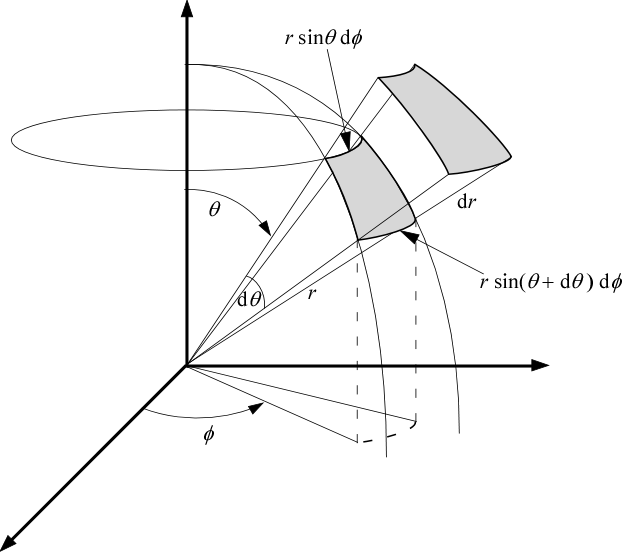
\includegraphics[width=0.6\textwidth]{images/control-volume-spherical.png}
    \caption{The control volume in spherical coordinates.}
    \label{fig:controlvolume}
\end{figure}

\section{Overview}

This document goes over the derivation of the continuity equation in spherical coordinates. 
In \S~\ref{sect:deriveterms}, we'll derive the individual terms of the continuity equation for spherical coordinates.
In \S~\ref{sect:combineterms}, we'll combine and simplify the terms into the continuity equations.

\subsection{Spherical Coordinate System}
    It is assumed that the reader is already knowledgeable as to the nature of spherical coordinate systems.
    For reference, the volume of a spherical differential element is given by equation~\ref{eq:diffvolume}.
    %
    \begin{equation}
        d\volume = r^2 \sin \theta dr d\theta d\phi
        \label{eq:diffvolume}
    \end{equation}

    In this document, the velocity components will be given as \(u_r,\ u_{\theta},\) and \(u_{\phi}\) for the radial (\(r\)), polar (\(\theta\)), and azimuthal (\(\phi\)) directions respectively.

\subsection{Continuity Equation}
    The basic continuity equation is simply the sum of the mass entering the control volume equals the time rate of change of the mass in the control volume. The base equation that will be used is thus:
    %
    \begin{equation*}
        \frac{\partial m}{\partial t} = \sum \dot{m}_i
    \end{equation*}

    The mass flows entering/exiting the control volume can be written as the product of the flux at the face of a control volume, \(\dot{m}''_{ij}\), and the area of said face, \(A_{ij}\):
    %
    \begin{equation}
        \frac{\partial m}{\partial t} = \sum \dot{m}''_{ij} A_{ij}
        \label{eq:base_equation}
    \end{equation}

    Here, \(i\) represents one of the three coordinate directions (\(r, \theta, \phi\)), and \(j\) represents the two opposite faces in the coordinate directions. We assume the flow is moving in the positive coordinate directions exclusively, so \(j\) can be thought of as the mass flow going in and mass flow going out.

    This turns equation~\ref{eq:base_equation} into:
    %
    \begin{equation}
        \frac{\partial m}{\partial t} + 
        \sum_{i=r, \theta, \phi}
        (\dot{m}''_{i,out} A_{i,out} - \dot{m}''_{i,in} A_{i,in}) = 0 
        \label{eq:base_equation_full}
    \end{equation}

    % \begin{equation}
    %     \frac{\partial m}{\partial t} + 
    %     (\dot{m}''_{r,out} A_{r,out} - \dot{m}''_{r,in} A_{r,in}) + 
    %     (\dot{m}''_{\theta,out} A_{\theta,out} - \dot{m}''_{\theta,in} A_{\theta,in}) + 
    %     (\dot{m}''_{\phi,out} A_{\phi,out} - \dot{m}''_{\phi,in} A_{\phi,in}) = 0
    %     \label{eq:base_equation}
    % \end{equation}

\subsection{Other Information} \label{sect:otherinfo}
Many of the faces of the control volume can be simplified to a trapezoid. The area of a trapezoid is given as the product of the average of the two midsection sides, \(l_{short} + l_{long}\), and the height of the trapezoid, \(h\):
%
\begin{equation}
    A_{trapezoid} = \tfrac{1}{2} (l_{short} + l_{long}) \times h
    \label{eq:traparea}
\end{equation}

The order of differential terms is used extensively in this document. To summarize, whenever you have a differential term, such as \(dr\), raised to a higher order, you assume it is equal to zero. This is sort of a reverse l'Hopital's rule, where as a function goes to infinity, the lower order terms dominate over higher order terms.

\section{Deriving Individual Terms} \label{sect:deriveterms}
We'll first start with the defining the the four components of the continuity equation.

    \subsection{Mass Time Rate of Change}
        \begin{equation*}
            \frac{\partial m}{\partial t} = \frac{\partial \rho}{\partial t}d\volume
        \end{equation*}

        \begin{equation}
            \frac{\partial m}{\partial t} = 
            \frac{\partial \rho}{\partial t} r^2 \sin\theta dr d\theta d\phi
            \label{eq:dm/dt}
        \end{equation}

    \subsection{Radial Mass Flow}
        \subsubsection{Radial Mass Flux}
            \begin{equation}
                \dot{m}_{r,in}'' = \rho u_r
            \end{equation}
            %
            \begin{equation}
                \dot{m}_{r,out}'' = \rho u_r  +
                \frac{\partial \rho u_r}{\partial r} dr
            \end{equation}

        \subsubsection{Radial Face Areas}
        \paragraph{Inlet}

            The faces in the radial direction form a trapezoid, so we use equation~\ref{eq:traparea} to calculate it's area.
            \begin{equation*}
                l_{short} = r\sin(\theta) d\phi  \qquad
                l_{long} = r\sin(\theta + d\theta) d\phi
            \end{equation*}
            \begin{equation}
                A_{r,in} = \tfrac{1}{2} [r\sin(\theta) d\phi + r\sin(\theta + d\theta) d\phi] \times rd\theta
                \label{eq:Arin_init}
            \end{equation}

            Using \(\sin(A+B) = \sin A \cos B + \sin B \cos A \), we can expand the \(\sin (\theta + d\theta)\) term. We then also state that as \(d\theta \rightarrow 0\):
            \begin{equation*}
                \sin (d\theta) \approx d\theta \qquad \cos(d\theta) \approx 1
            \end{equation*}
            therefore we get the following:
            \begin{equation*}
                \sin(\theta+d\theta) = 
                \sin\theta \cos d\theta + \sin d\theta \cos\theta \approx
                \sin\theta + \cos\theta d\theta
            \end{equation*}

            Substituting this into equation~\ref{eq:Arin_init} and reorganizing terms, we get the following:
            \begin{equation*}
                \text{Eqn.}\ \ref{eq:Arin_init} \Rightarrow
                r^2\sin\theta d\theta d\phi + \tfrac{1}{2}r^2\cos \theta d\theta^2 d\phi
            \end{equation*}

            We assume \(d\theta^2 \approx 0\) (see \S \ref{sect:otherinfo}), which gives us:
            \begin{equation}
                A_{r,in} = r^2 \sin\theta d\theta d\phi
                \label{eq:Arin_final}
            \end{equation}

        \paragraph{Outlet}
            The outlet face is done identically to the inlet face.
            \begin{equation*}
                l_{short} = (r + dr)\sin(\theta) d\phi  \qquad
                l_{long} = (r + dr)\sin(\theta + d\theta) d\phi
            \end{equation*}
            \begin{equation}
                A_{r,out} = \tfrac{1}{2} [(r + dr)\sin(\theta) d\phi + (r + dr)\sin(\theta + d\theta) d\phi] \times (r + dr)d\theta
                \label{eq:Arout_init}
            \end{equation}
            \begin{equation*}
                \Rightarrow
                \tfrac{1}{2} (r + dr)^2 [ \sin\theta + \sin (\theta + d\theta)] d\theta d\phi
            \end{equation*}

            Substituting the same trig identity as in `Inlet' and expanding \((r + dr)^2\), and dropping higher order differential terms, we get:
            \begin{equation*}
                \tfrac{1}{2} (r^2 + 2rdr + \cancelto{0}{dr^2}) [\sin\theta d\theta d\phi + \cos\theta \cancelto{0}{d\theta^2} d\phi]
                \Rightarrow \tfrac{1}{2} (r^2 + 2rdr) \sin\theta d\theta d\phi
            \end{equation*}

            \begin{equation}
                \therefore\quad A_{r,out} = r^2 \sin\theta d\theta d\phi + 
                2r\sin\theta drd\theta d\phi
                \label{eq:Arout_final}
            \end{equation}

        \subsubsection{Combining Radial Flow Terms}
            \begin{multline*}
                \dot{m}_r = (\dot{m}''_{r,out} A_{r,out} - \dot{m}''_{r,in} A_{r,in}) 
                \\\Rightarrow
                \left(\rho u_r  + \frac{\partial \rho u_r}{\partial r} dr\right)\left(r^2 \sin\theta d\theta d\phi + 2r\sin\theta dr d\theta d\phi\right) -
                \left(\rho u_r\right)\left(r^2 \sin\theta d\theta d\phi\right)
            \end{multline*}
            Expanding out the terms, we find that the first and last terms cancel each other out and that a \(dr^2\) appears:
            \begin{multline*}
                \Rightarrow
                \cancel{\rho u_r r^2 \sin\theta d\theta d\phi} +
                \frac{\partial \rho u_r}{\partial r} r^2 \sin\theta dr d\theta d\phi +
                2\rho u_r r\sin\theta dr d\theta d\phi + \\
                \frac{\partial \rho u_r}{\partial r} 2r\sin\theta \cancelto{0}{dr^2} d\theta d\phi - 
                \cancel{\rho u_r r^2 \sin\theta d\theta d\phi}
            \end{multline*}

            \begin{equation}
                \dot{m}_r = \frac{\partial \rho u_r}{\partial r} r^2 \sin\theta dr d\theta d\phi +
                2\rho u_r r\sin\theta dr d\theta d\phi
                \label{eq:mdotr}
            \end{equation}


\section{Combining Terms} \label{sect:combineterms}


\end{document}